\documentclass[acmtog, authorversion]{templates/acmart}

%%%%% Status Meaning %%%%%
% internal             = 0
% submission           = 1
% revision             = 2
% camera-ready         = 3
% camera-ready-author  = 4
\newcommand{\status}{4}

\setcopyright{acmcopyright}
\copyrightyear{2022}
\acmJournal{TOG}
\acmYear{2022}
\acmVolume{41}
\acmNumber{6}
\acmArticle{1}
\acmDOI{}
\acmSubmissionID{XXX-XXX-XXX}
\citestyle{acmauthoryear}

%% The "title" command has an optional parameter,
%% allowing the author to define a "short title" to be used in page headers.
%% \title[short title]{full title}
%% Capitalize your title: https://capitalizemytitle.com/
\title{The Name of the Title is Hope}

%% The "author" command and its associated commands are used to define
%% the authors and their affiliations.
%% Of note is the shared affiliation of the first two authors, and the
%% "authornote" and "authornotemark" commands
%% used to denote shared contribution to the research.
\author{Ben Trovato}
\authornote{Both authors contributed equally to this research.}
\email{trovato@corporation.com}
\orcid{1234-5678-9012}
\author{G.K.M. Tobin}
\authornotemark[1]
\email{webmaster@marysville-ohio.com}
\affiliation{%
  \institution{Institute for Clarity in Documentation}
  \streetaddress{P.O. Box 1212}
  \city{Dublin}
  \state{Ohio}
  \country{USA}
  \postcode{43017-6221}
}

\author{Lars Th{\o}rv{\"a}ld}
\affiliation{%
  \institution{The Th{\o}rv{\"a}ld Group}
  \streetaddress{1 Th{\o}rv{\"a}ld Circle}
  \city{Hekla}
  \country{Iceland}}
\email{larst@affiliation.org}

\author{Valerie B\'eranger}
\affiliation{%
  \institution{Inria Paris-Rocquencourt}
  \city{Rocquencourt}
  \country{France}
}

\author{Aparna Patel}
\affiliation{%
 \institution{Rajiv Gandhi University}
 \streetaddress{Rono-Hills}
 \city{Doimukh}
 \state{Arunachal Pradesh}
 \country{India}}

\author{Huifen Chan}
\affiliation{%
  \institution{Tsinghua University}
  \streetaddress{30 Shuangqing Rd}
  \city{Haidian Qu}
  \state{Beijing Shi}
  \country{China}}

\author{Charles Palmer}
\affiliation{%
  \institution{Palmer Research Laboratories}
  \streetaddress{8600 Datapoint Drive}
  \city{San Antonio}
  \state{Texas}
  \country{USA}
  \postcode{78229}}
\email{cpalmer@prl.com}

\author{John Smith}
\affiliation{%
  \institution{The Th{\o}rv{\"a}ld Group}
  \streetaddress{1 Th{\o}rv{\"a}ld Circle}
  \city{Hekla}
  \country{Iceland}}
\email{jsmith@affiliation.org}

\author{Julius P. Kumquat}
\affiliation{%
  \institution{The Kumquat Consortium}
  \city{New York}
  \country{USA}}
\email{jpkumquat@consortium.net}

%% By default, the full list of authors will be used in the page
%% headers. Often, this list is too long, and will overlap
%% other information printed in the page headers. This command allows
%% the author to define a more concise list
%% of authors' names for this purpose.
\renewcommand{\shortauthors}{Trovato and Tobin, et al.}

%%
%% The code below is generated by the tool at http://dl.acm.org/ccs.cfm.
%% Please copy and paste the code instead of the example below.
%%
\begin{CCSXML}
<ccs2012>
 <concept>
  <concept_id>10010520.10010553.10010562</concept_id>
  <concept_desc>Computer systems organization~Embedded systems</concept_desc>
  <concept_significance>500</concept_significance>
 </concept>
 <concept>
  <concept_id>10010520.10010575.10010755</concept_id>
  <concept_desc>Computer systems organization~Redundancy</concept_desc>
  <concept_significance>300</concept_significance>
 </concept>
 <concept>
  <concept_id>10010520.10010553.10010554</concept_id>
  <concept_desc>Computer systems organization~Robotics</concept_desc>
  <concept_significance>100</concept_significance>
 </concept>
 <concept>
  <concept_id>10003033.10003083.10003095</concept_id>
  <concept_desc>Networks~Network reliability</concept_desc>
  <concept_significance>100</concept_significance>
 </concept>
</ccs2012>
\end{CCSXML}

\ccsdesc[500]{Computer systems organization~Embedded systems}
\ccsdesc[300]{Computer systems organization~Redundancy}
\ccsdesc{Computer systems organization~Robotics}
\ccsdesc[100]{Networks~Network reliability}

%%
%% Keywords. The author(s) should pick words that accurately describe
%% the work being presented. Separate the keywords with commas.
\keywords{datasets, neural networks, gaze detection, text tagging}

%%% Language %%%%
\RequirePackage[english]{babel}                  % Hyphenation and date format
\RequirePackage{xspace}                          % Abbreviation spacing
\RequirePackage{xpunctuate}                      % Abbreviation spacing

%%% Tex-scripting %%%
\RequirePackage{ifthen}                          % If-then-else latex logic
\RequirePackage{soul}                            % Underlining and Strike-through
\RequirePackage{xargs}                           % For \newcommandx

%%% Color %%%
\RequirePackage{color}                           % Draft annotation coloring

%%% Math-mode %%%
\RequirePackage{amsmath}                         % Math equations
\RequirePackage{bm}                              % Math bold symbols

%%% Cross-referencing %%%
\RequirePackage[toc,page,titletoc]{appendix}     % Appendix section
\RequirePackage[capitalize,nameinlink]{cleveref} % Easy to use cross-referencing
\crefname{supp}{Supplement}{Supplements}     % Supplement section name setting

%%% Figures %%%
\RequirePackage{caption}                         % Figure captions
\RequirePackage{subfig}                          % Nested figures

%
% Colors
%
\definecolor{INCOMPLETECOLOR}{RGB}{178,34,34}
\definecolor{UNDERREVISIONCOLOR}{RGB}{210,121,121}
\definecolor{FEEDBACKNEEDEDCOLOR}{RGB}{230,170,50}
\definecolor{FEEDBACKGIVENCOLOR}{RGB}{121,210,121}
\definecolor{COMPLETECOLOR}{RGB}{121,124,210}
\definecolor{LOCKEDCOLOR}{RGB}{153,102,255}

\definecolor{TODOCOLOR}{RGB}{255,0,0}
\definecolor{MONDECOLOR}{RGB}{0,0,255}
\definecolor{QICOLOR}{RGB}{118,185,0}
\definecolor{ANJULCOLOR}{RGB}{127,127,0}
\definecolor{RACHELCOLOR}{RGB}{127,0,127}
\definecolor{GUESTCOLOR}{RGB}{0,127,127}

\definecolor{WHITE}{RGB}{255,255,255}

%
% Global macros
%
\newcommand{\nothing}[1]{}
\newcommand{\isolated}[1]{\hfill\break#1\xspace}
\newcommand{\Caption}[2]{\caption[#1]{{\em #1} #2}}
\newcommand{\Quote}[1]{{``#1''}}

\newcommand{\Ie}{{I.e.,}\xspace}
\newcommand{\ie}{{i.e.,}\xspace}
\newcommand{\Eg}{{E.g.,}\xspace}
\newcommand{\eg}{{e.g.,}\xspace}
\newcommand{\etal}{{et~al\xperiod}\xspace}
\newcommand{\aka}{{a.k.a.,}\xspace}
\newcommand{\etc}{{etc\xperiod}\xspace}
\newcommand{\cf}{{cf\xperiod}\xspace}

%
% Adding Comments
%
\ifthenelse{\equal{\status}{0}} {                     % INTERNAL Version

    \newcommand{\todo}[1]{%
        \addcontentsline{toc}{subsection}{%           %
            \protect\numberline{}%                    % Align text appropriately
            \textcolor{TODOCOLOR}{[TODO] #1}}%        % Add todo to the table of contents
            \textcolor{TODOCOLOR}{[TODO] \emph{#1}}}% % Typeset the todo note in the text
    \newcommand{\warning}[1]{\todo{#1}}
    \newcommand{\note}[1]{{\it\color{blue} #1}}

    \newcommand{\todolist}{\newpage\tableofcontents}

    % Usage: \monde[(OPTIONAL) Text to underline]{Comment.}
    \newcommandx{\monde}[2][1=]
        {\setulcolor{MONDECOLOR}{\ul{#1}}
         \isolated{\textcolor{MONDECOLOR}{\textbf{Monde:} #2}}}
    \newcommandx{\qisun}[2][1=]
        {\setulcolor{QICOLOR}{\ul{#1}}
         \isolated{\textcolor{QICOLOR}{\textbf{Qi:} #2}}}
    \newcommandx{\anjul}[2][1=]
        {\setulcolor{ANJULCOLOR}{\ul{#1}}
         \isolated{\textcolor{ANJULCOLOR}{\textbf{Anjul:} #2}}}
    \newcommandx{\rachel}[2][1=]
        {\setulcolor{RACHELCOLOR}{\ul{#1}}
         \isolated{\textcolor{RACHELCOLOR}{\textbf{Rachel:} #2}}}

    % Usage: \guest[(OPTIONAL) Text to underline]{Name}{Comment.}
    \newcommandx{\guest}[3][1=]
        {\setulcolor{LOCKEDCOLOR}{\ul{#1}} \textcolor{LOCKEDCOLOR}
        {[\textbf{#2:} #3]}}
}{                                                    % NON-INTERNAL Versions
    \newcommand{\todo}[1]{}
    \newcommand{\warning}[1]{}
    \newcommand{\note}[1]{}
    \newcommand{\todolist}{}
    \newcommandx{\monde}[2][1=]{#1}
    \newcommandx{\qisun}[2][1=]{#1}
    \newcommandx{\anjul}[2][1=]{#1}
    \newcommandx{\rachel}[2][1=]{#1}
    \newcommandx{\guest}[3][1=]{#1}
}

%
% Revision Annotation
% Usage: \revise{Text to delete.}{Text to insert.}
%

\ifthenelse{\equal{\status}{0}} {          % INTERNAL Version
    % Highlight revised text.
    % Strike-through deleted text
    \newcommand{\revise}[2]{\textcolor{INCOMPLETECOLOR}{\st{#1}}\textcolor{blue}{#2}}
}{}
\ifthenelse{\equal{\status}{1}} {          % SUBMISSION Version
    \newcommand{\revise}[2]{#2}
}{}
\ifthenelse{\equal{\status}{2}} {          % REVISION Version
    % Highlight revised text.
    \newcommand{\revise}[2]{\textcolor{blue}{#2}}
}{}
\ifthenelse{\equal{\status}{3}} {          % CAMERA-READY Version
    \newcommand{\revise}[2]{#2}
}{}
\ifthenelse{\equal{\status}{4}} {          % CAMERA-READY AUTHOR Version
    \newcommand{\revise}[2]{#2}
}{}

%
% Status Badges
%
\ifthenelse{\equal{\status}{0}} {
    \newcommand{\badge}[2]{\colorbox{#1}{\small\textcolor{WHITE}{\texttt{#2}}}}
    \newcommand{\headerBadge}[2]{\hspace*{\fill}\badge{#1}{#2}}
    \newcommand{\locked}{\headerBadge{LOCKEDCOLOR}{locked}}
    \newcommand{\complete}{\headerBadge{COMPLETECOLOR}{complete}}
    \newcommand{\feedbackGiven}{\headerBadge{FEEDBACKGIVENCOLOR}{feedback given}}
    \newcommand{\feedbackNeeded}{\headerBadge{FEEDBACKNEEDEDCOLOR}{feedback needed}}
    \newcommand{\underRevision}{\headerBadge{UNDERREVISIONCOLOR}{under revision}}
    \newcommand{\incomplete}{\headerBadge{INCOMPLETECOLOR}{incomplete}}
}{
    \newcommand{\badge}[2]{}{}
    \newcommand{\headerBadge}[2]{}{}
    \newcommand{\locked}{}
    \newcommand{\complete}{}
    \newcommand{\feedbackGiven}{}
    \newcommand{\feedbackNeeded}{}
    \newcommand{\underRevision}{}
    \newcommand{\incomplete}{}
}

\newcommand{\energy}{E}
\newcommand{\mass}{m}
\newcommand{\lightspeed}{c}

%%% Supplementary material configuration %%%
%%% Makefile automatically manages this line. DO NOT EDIT.
%%% When commented supplement is rendered and vice versa.
% \includeonly{}
%%% Supplementary material configuration %%%

\begin{document}

% Main
\begin{teaserfigure}
  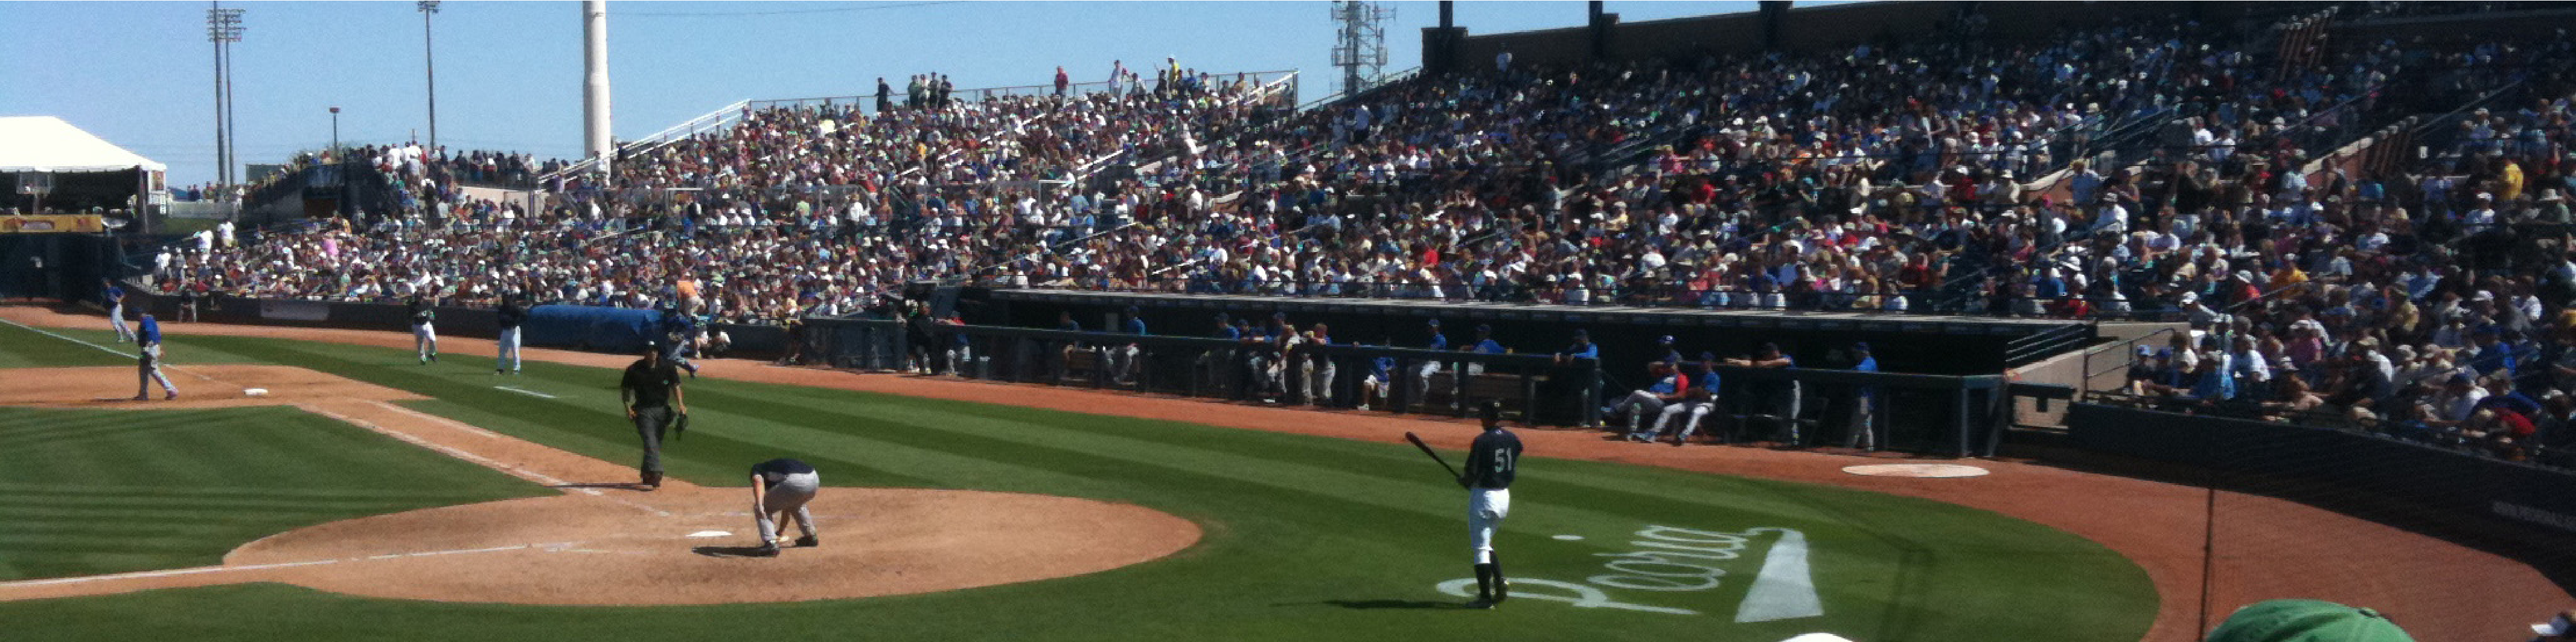
\includegraphics[width=\textwidth]{assets/sampleteaser}
  \caption{Seattle Mariners at Spring Training, 2010.}
  \Description{
      Enjoying the baseball game from the third-base seats.
      Ichiro Suzuki preparing to bat.
  }
  \label{fig:teaser}
\end{teaserfigure}


\begin{abstract}
    Writing papers and managing projects are essential for conducting research.
A research paper describes the final outcomes, but can also help manage intermediate progress.
This document provides a template for writing papers and describes how to manage projects via drafts.

Start the abstract when you have some rough ideas, before they are forgotten amid your busy lives.
It does not need to be fancy, as long as you can understand your own writing later.
The eventual abstract should be the minimalist version of the entire paper, with key information outlined in the introduction.
\end{abstract}

\maketitle

\todolist

\section{Introduction \incomplete}
\label{sec:introduction}

\note{
What problem we are trying to solve.
Why it is important, and why people should care.
}%note

Writing research documents, such as conference/journal/white papers, patent applications, grant proposals, and course reports, is a core activity for many poor souls including professors, researchers, engineers, and students.
Since we must do it one way or another, sooner or later, we might as well do it as happily and effectively as possible.
This document is meant to document both my experience of learning this process and also share my findings on effective writing advice and general project management.
Note that large portions of this document has been inherited from my advisers and mentors and developed further (see Acknowledgements).

\note{
What prior works have done, and why they are not adequate.
(Note: this is just high level big ideas. Details should go to a previous work section.)
}%note

Some people, including very successful ones, write papers only at the end of a project, like days if not hours prior to a submission deadline.
This almost always leads to total chaos and breakdown, unless you have other means to keep track and organize all the relevant pieces of information.

\note{
What our method has to offer, sales pitch for concrete benefits, not technical details.
Imagine we are doing a TV advertisement here.
}%note

This document provides a template for writing research papers, and describes how to manage project progress via iterating drafts.
Doing this correctly can help you achieve productive research and a happy life, e.g. working anywhere anytime without synchronous meetings with your collaborators.

\note{
Our main idea, giving people a take home message and (if possible) see how clever we are.
}%note

I learned from my PhD adviser to start writing from the moment I have the faintest idea, and gradually update the drafts to reflect progress.
Coming from a software engineering background, I was aware of how revision control is essential for sharing and editing source files, especially among large groups of collaborators.
The iterative nature of writing and coding matches well with the capability of revision control.
Thus I prefer Latex + git/svn (e.g. github, bitbucket, and the svn server under my hosting service), even though I can still manage with MS Word + cloud drive (e.g. Google drive, Box, and Dropbox). 
A good computer scientist writes papers like programs, and manages Latex files like source codes.
These repos are external memories and communication mediums for the collective brains of my teams.

\note{
Our algorithms and methods to show technical contributions and that our solutions are not trivial.
}%note

\begin{figure}
  \centering
  \includegraphics[width=\linewidth]{example-image-a}
  \Caption{
      Figure title.
  }{
      More detailed description of figure.
  }
  \Description{Description of figure.}
  \label{fig:example}
\end{figure}


Translating thoughts into words, diagrams, equations, pseudo-codes, or codes is a good way to clarify and consolidate.
If you are writing a graphics/HCI paper, design the figures so that they alone can provide a high level picture of the main points.
As exemplified in \Cref{fig:example}, a figure can contain images, drawings, or combinations. 

\note{
Results, applications, and extra benefits.
}%note

You can use the associated files as a starting template for your research papers.
Start with the \texttt{Makefile}, and notice the two build targets: final for official submission and public disclosure, and draft for internal sharing among your collaborators (including yourself).

\section{Related Work \underRevision}
\label{sec:related}

Cite all relevant works, and how yours stands on the shoulder of these previous giants.
\todo{Add more citations.}
\monde[Use a BibTeX file such as \texttt{paper.bib} and you can cite relevant works such as \mbox{\cite{Duinkharjav2022GazeTiming}}.]
{Here's a comment on for this line.}

\section{Method \feedbackNeeded}
\label{sec:method}

Written words are more concrete than ideas in your head.
Math equations and pseudo-codes are even more concrete than words, and can help, even though not essential, for exposition.
Programs that produce the actual results are the most concrete, but the amount and level of information is not suitable for a research paper.
I like to write down math and pseudo-code first as a way to design the algorithms before actual implementation.

\subsection{Math}
\label{sec:method:math}

\begin{align}
\energy = \mass \lightspeed^2
\label{eqn:emc2}
\end{align}

Always use defined instead of naked math symbols for clarify and consistency.
For example, in \Cref{eqn:emc2} I define all symbols inside \texttt{symbols.tex} so later if I need to change $\energy$ from $E$ to $e$ I just need to change one line in \texttt{symbols.tex} instead of chasing $E$ everywhere.
This can save you a lot of time and sanity if you have many math symbols.

\section{Results \feedbackGiven}
\label{sec:result}

Provide evaluation, analysis, comparisons, demos, and applications.

You can more concretely learn everything I described in this document by apprenticing some research projects with me.

\section{Limitations and Future Work \complete}
\label{sec:future-work}

Disclose all limitations, and describe how potential future works can address these and lead to more interesting and ground breaking stuff.

I am continuously updating this document based on your questions and feedbacks.

I believe in the (near?) future all research papers, at least in computer science, will be published in a form that contains everything in one place, including math, code, and data, so that readers can parse the descriptions and repeat the experiments, like what we can do with Jupyter/Ipython notebooks today.

\begin{table}
  \caption{Frequency of Special Characters}
  \label{tab:freq}
  \begin{tabular}{ccl}
    \toprule
    Non-English or Math&Frequency&Comments\\
    \midrule
    \O & 1 in 1,000& For Swedish names\\
    $\pi$ & 1 in 5& Common in math\\
    \$ & 4 in 5 & Used in business\\
    $\Psi^2_1$ & 1 in 40,000& Unexplained usage\\
  \bottomrule
\end{tabular}
\end{table}




\begin{acks}
    To Robert, for the bagels and explaining CMYK and color spaces.
\end{acks}

% Bibliography
\bibliographystyle{templates/acmart}
\bibliography{bibliography}

% Supplementary material
% Uncomment next line to make a one-column supplement
% \onecolumn

\section{How to use this template}

This \LaTeX{} template was developed to (1) streamline collaborative manuscript editing and (2) automate many processes that manu\-scripts undergo throughout the publication process of academic papers.
Many ideas, features, and aspects in this template were adapted from my previous collaborators and mentors such as Qi Sun, Li-Yi Wei and Jane Hoffswell.

\subsection{Usage}

The \LaTeX{} compilation is managed by a \texttt{Makefile}.
The \texttt{Makefile} features multiple build targets meant for various versions of the document, such as \texttt{internal} for sharing between collaborators, and \texttt{submission} for anonymous submissions.
These targets are built by running \texttt{make <target\_name>} (\eg \texttt{make internal}).
See \Cref{sec:howto:build-pipeline} for details on the various build targets.

\paragraph{Pre-requisites}
The \texttt{Makefile} assumes the usage of \texttt{pdflatex}, so please make sure to install the \texttt{texlive}, \texttt{texlive-latex-extra}, \texttt{texlive-fonts-recommended}, \texttt{texlive-science}, and \texttt{texlive-x\hfill\break string} packages.
Additionally, \texttt{ghostscript} is used for post-com\-pilation PDF document processing such as to separate the document into separate files for the manuscript and supplementary materials.
See more details on this in \Cref{sec:howto:build-pipeline}.

\subsection{\LaTeX{} macros for collaborative editing}
\label{sec:howto:macros}

This template features a number of very convenient macros designed to make collaborative writing much easier and more streamlined.
All of these macro definitions can be found in \texttt{conf/macros.tex} and edited as necessary.
Below, we outline what the features are and how to use them.

\paragraph{Tracking Progress: Status Badges and To-do Items}
When collaborating on a large document, it's often helpful to keep track of what sections have been reviewed, what sections are complete \etc
This template enables status tracking of paper sections via \emph{Status Badges} as well as \emph{To-do Item} annotations which can be viewed in summary at the top of the document.

\emph{Status Badges} indicate what state a particular section of the manuscript is in and allows collaborators to claim, and release sections as necessary.
To add a badge to a section, simply add the corresponding badge command at the end of the section title
(\eg \texttt{\textbackslash section\{Section Title \textbackslash incomplete\}}).
This badge will not only annotate the section title with its corresponding status, but also include the annotation to a summary \Quote{table-of-contents} which appears at the top of the document when rendered in the \texttt{internal} version.
For the full list of possible status badges, see \Cref{tab:howto:status-badges}.
%
\begin{table}[ht]
    \caption{Status badges}
    \label{tab:howto:status-badges}
    \begin{tabular}{ll}
        \toprule
        Command & Created Badge\\
        \midrule
        \texttt{\textbackslash incomplete} & \incomplete\\
        \texttt{\textbackslash underRevision} & \underRevision\\
        \texttt{\textbackslash feedbackNeeded} & \feedbackNeeded\\
        \texttt{\textbackslash feedbackGiven} & \feedbackGiven\\
        \texttt{\textbackslash complete} & \complete\\
        \texttt{\textbackslash locked} & \locked\\
        \bottomrule
    \end{tabular}
\end{table}

\emph{To-do Items} are also a helpful tool for annotating important to-do items that need to be tracked.
Including an actionable in the source document as \texttt{\textbackslash todo\{revise this sentence\}} will render the to-do item within the manuscript in a highlighted red color, and also include a copy of this to-do item in the \Quote{table-of-contents} at the top of the document just like the \emph{Status Badges}.

The combination of these two macros can help collaborators keep track of everything that still needs to be done for a paper submission prior to deadlines.

\paragraph{Exchanging feedback via in-document comments}
In addition to important to-do items, sometimes it is helpful to simply have asynchronous discussions that aren't necessarily mission critical within the document draft itself.
To facilitate this workflow, the template also supports macros for in-document comments by multiple collaborators, each highlighted in a different color.
\monde{For example, I might have some thoughts on the organization of this section.}
\qisun{And I might respond to Monde's concerns in response.}

The current template has pre-defined macros for four collaborators: \texttt{monde}, \texttt{qi}, \texttt{anjul}, and \texttt{rachel}.
To use the macro call the macro as \texttt{\textbackslash monde\{comment contents\}} for a simple comment.
\monde[To annotate existing text to reference by the comment,]{like this,}\break
put the existing text into square brackets.
For example, \texttt{\textbackslash monde[anno\hfill\break tated text]\{comment contents\}}.
There is also a generic \texttt{guest} command to allow a guest to input their name into their comment without having to define a new macro.
To use this version, call the macro as \texttt{\textbackslash guest\{name\}\{comment contents\}} for a simple comment and \texttt{\textbackslash guest[annotated text]\{name\}\{comment contents\}} for annotated comments.

\paragraph{Revision annotation}
During the revision stage of a document for publication, reviewers often ask for specific edits to the manuscript.
To enable an easy back and forth between the reviewer and the authors, highlighting all the changed text can be very helpful.
To this end, this template features a \texttt{\textbackslash revise\{text to remove\}\{text to add\}} macro which annotates both removed and added text.
By inputting the to-be-removed text in the first argument, and the to-be-added text in the second argument, the annotation \revise{won't}{will} look like this.
By default, the removed text will only be shown in the \texttt{internal} version of the document, while the \texttt{revision} version of the document only shows the added text.
But you can edit this behavior in the \texttt{conf/macros.tex} file.
The automated build pipeline (\cf \Cref{sec:howto:build-pipeline}) allows seamless changes between the different versions of how a revised text should be rendered.

\subsection{File Organization}

This template is organized into a granular structure and logical separation of various types of source files that make up a \LaTeX{} document.
\Cref{tab:howto:path-description} explains what types of files are at the various paths.
%
\begin{table}[ht]
    \caption{File paths and their functions}
    \label{tab:howto:path-description}
    \begin{tabular}{ll}
        \toprule
        Path & Function\\
        \midrule
        \texttt{sections} & numbered section \LaTeX{} source files\\
        \texttt{sections/abstract.tex} & document abstract\\
        \texttt{sections/acks.tex} & acknowledgements section\\
        \texttt{sections/document.tex} & manuscript sections entry point\\
        \texttt{sections/readme.tex} & how to use this template\\
        \texttt{sections/supp.tex} & supp. material entry point\\
        \texttt{tables} & table \LaTeX{} source files\\
        \texttt{figures} & figure \LaTeX{} source files\\
        \texttt{assets} & illustrations and plots\\
        \texttt{conf} & \LaTeX{} configurations\\
        \texttt{metadata} & metadata of the document\\
        \texttt{targets} & \LaTeX{} compilation entry points\\
        \texttt{paper.tex} & combination of source files\\
        \texttt{paper.bib} & bibliography\\
        \texttt{Makefile} & build pipeline definitions\\
        \texttt{build} & build outputs\\
        \bottomrule
    \end{tabular}
\end{table}

\paragraph{Sections}
All numbered sections are combined in \texttt{sections/docu\hfill\break ment.tex}, which in turn are inputted in the compilation process in \texttt{paper.tex}.
Each numbered section name is prepended by its number for visual clarity, and each section is given its \LaTeX{} label in the form \texttt{\textbackslash label\{sec:<section\_name>\}}.
Further subsection labels are nested as \texttt{sec:<section\_name>:<subsection\_name>}.

\paragraph{Tables and Figures}
All table and figure source files are separated from \emph{Section} source files to enable easy edits to where a figure should be added in the source.
Each figure is given its \LaTeX{} label in the form \texttt{\textbackslash label\{tab:<table\_name>\}} or \texttt{\textbackslash label\{fig:figure\_name\}}

\paragraph{Packages, Aliases, and Macros}
\LaTeX{} package imports are consolidated in \texttt{conf/packages.tex}.
To avoid complications when some packages need to be deprecated in the future, it's advised that the specific usage of each package is documented as a comment.
For example, we use the \texttt{soul} package to enable underlining and strike-through functionality for annotating collaborator comments, and text revisions.
If in the future, either this feature of the template is changed or removed, removing this package dependency will be much easier to identify and execute.

All symbol aliases used during writing are consolidated within \texttt{conf/symbols.tex}, while more complex macros are in \texttt{conf/macro\hfill\break s.tex}.
More details on what kind of macros are used in this template are in \Cref{sec:howto:macros}.

\paragraph{Paper metadata}
All source files pertaining to paper metadata, such as the title, authors, journal number, publication year \etc are included in \texttt{metadata/} and are self-explanatory.
These metadata fields are inserted into the compilation in \texttt{paper.tex}.
If you're changing the document class, include any document class related metadata fields in the \texttt{metadata/} directory, and change the organization of source files within \texttt{paper.tex}.

\paragraph{Build targets}
All build targets have their associated \LaTeX{} entry point inside \texttt{targets/} as well as a  \texttt{Makefile} target.
See more details about the build pipeline in \Cref{sec:howto:build-pipeline}.

\subsection{Build Pipeline}
\label{sec:howto:build-pipeline}

The build process of the manuscript is fully automated via a \texttt{Makefile} and allows the user to seamlessly produce different versions of the manuscript and supplementary materials documents.
\ie the document can be produced at various stages of \Quote{readiness for publication}, with each different stage revealing or hiding various comments and annotations.
The supported document stages are described in \Cref{tab:howto:doc-stages}.
%
\begin{table}[ht]
    \caption{Document stages and their usage and features.}
    \label{tab:howto:doc-stages}
    \begin{tabular}{ll}
        \toprule
        Build target & Usage and features\\
        \midrule
        \texttt{internal} & internal collaborative use with comments shown\\
        \texttt{submission} & anonymous submission with no annotations\\
        \texttt{revision} & annotated anonymous revision for reviewers\\
        \texttt{camready} & final camera-ready with author names shown\\
        \texttt{camauthor} & author-version for sharing post-publication\\
        \bottomrule
    \end{tabular}
\end{table}

You may add additional document stages by
%
\begin{itemize}
    \item adding a new \LaTeX compilation entry file inside \texttt{targets/},
    \item updating the \texttt{Makefile} targets, and
    \item adding your custom logic for what annotations to enable in \texttt{conf/macros.tex}.
\end{itemize}

\paragraph{Automated manuscript and supp. material separation}
Often a paper publication requires an associated supplementary materials section for any exposition that does not central to the publication and are omitted from the main manuscript.
In order to take advantage of \LaTeX{} cross-referencing features, such as \texttt{\textbackslash Cref}, it's best to compile all the source files in one batch and generate a single PDF output.
However, doing so requires post-processing on the outputted file to separate them into multiple PDFs via an external application such as Adobe Acrobat \etc
Additionally, many paper templates also print the number of pages of the document which include the supplementary material pages if this method is used to generate two separate files for the main manuscript and the supplementary material.

This template takes care of these manual steps and also solves the page count issue and keeps all the complexity of the compilation and post-processing logic tucked away in the \texttt{Makefile}.
In order to take advantage of this feature, make sure to use the Makefile to compile your document and have its dependent \texttt{ghostscript} package installed on your machine.

\subsection{Future Features}
\label{sec:howto:future-features}

I'm constantly updating this template to help make the paper authoring and collaboration process more streamlined.
Below is a short list of features that I'm looking to add in the future:
%
\begin{itemize}
    \item add easy to use \LaTeX{} linting and formatting scripts;
    \item add helper scripts which \Quote{commit/revert} the revisions by stripping the \LaTeX{} tags and incorporating the existing revisions into the native text;
    \item add a \texttt{Makefile} target for preparing the publication for Arxiv upload;
    \item streamline the process of swapping out different style files;
    \item split the package dependencies so that unnecessary development / internal dependencies are omitted;
    \item add a script which \Quote{dumbs down} the \LaTeX{} source files into a single source file to satisfy strict publisher requirements.
\end{itemize}



\end{document}
